\clearpage
\chapter{Experiments}

\clearpage
\section{Mandelbrot}
Mandelbrot algorithm experiments were conducted using parameters presented in Tab. \ref{tab: MandelbrotParameters}. They describe amount of pixels generated and bitmap dimensions.
Sequential version of the algorithm had a MET  $\approx 5.6s$ . Parallel counterpart clocked at MET  $\approx 2.1s$, for a $\approx 62\%$ reduction. Parallel version with two \emph{Parallel.For} loops had a MET $\approx 2.7s$ which is $\approx 21\%$ slower than the less parallelized version using only one parallel loop. The best performing version using value type complex number had MET $\approx 1.9s$, for a $\approx 66\%$  reduction compared to sequential version and $\approx 11\%$  reduction to the parallel version. Additionaly, the value type version had 0 GC clean ups and virtually no (compared to others) memory consumption (Fig. \ref{fig: MandelbrotPerformance}, Tab. \ref{tab: MandelbrotBenchmarking}).

\begin{table}[!ht]
    \centering
    \caption{Mandelbrot benchmarking experiment parameters}
		\label{tab: MandelbrotParameters}
    \begin{tabular}{p{3cm}p{3cm}}
			\toprule
			\bfseries Name 	&
			\bfseries Value &
			\midrule
			Width & 2.5 \\
			Height & 2.5 \\
			Column amount & 4000 \\ 
			Row amount  & 4000 \\	
			\bottomrule
    \end{tabular}
\end{table}

\begin{figure}[!ht]
\centering
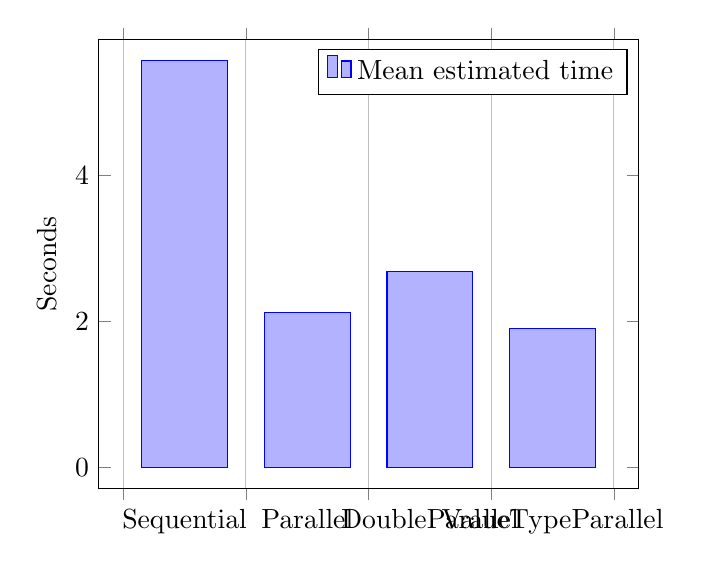
\begin{tikzpicture}
\begin{axis}[ symbolic x coords={
			Sequential, 
			Parallel, 
			DoubleParallel, 
			ValueTypeParallel, 
			DUMMY},
    xtick=data, 
		ylabel=Seconds,
    ybar interval=.7,
    enlargelimits=0.05]
    \addplot  coordinates {
      (Sequential, 5.576)
      (Parallel, 2.120)
      (DoubleParallel, 2.684)
      (ValueTypeParallel,1.903)
      (DUMMY, 0)
    };
     \legend{Mean estimated time}
\end{axis}
\end{tikzpicture}
\caption{Mandelbrot algorithm performance}
\label{fig: MandelbrotPerformance}
\end{figure}

\begin{sidewaystable}[!ht]
    \centering
    \caption{Mandelbrot benchmarking results}
		\label{tab: MandelbrotBenchmarking}
    \begin{tabular}{lp{3cm}p{1.5cm}p{1.5cm}p{2cm}p{2cm}p{2cm}p{2cm}}
			\toprule
			\bfseries Version 	&
			\bfseries Mean    	&
			\bfseries Error	    &
			\bfseries StdDev	  &
			\bfseries Gen 0	    &
			\bfseries Gen 1	    &
			\bfseries Gen 2	    &
			\bfseries Allocated &
			\midrule 
			Sequential & 5.576 s & 0.0564 s & 0.0528 s & 2483000 & 1000 & 1000 & 19851 MB \\ 
			Parallel & 2.120 s & 0.0458 s & 0.1350 s & 2485000 & 6000 & 1000 & 19843 MB \\ 
			DoubleParallel & 2.684 s & 0.0553 s & 0.1632 s & 2487000 & 39000 & 2000 & 19852 MB \\ 
			ValueTypeParallel & 1.903 s & 0.0137 s & 0.0128 s & 0 & 0 & 0 & 46 MB \\ 
			\bottomrule
    \end{tabular}
\end{sidewaystable}